\documentclass[a4paper,12pt]{article}
%\documentclass[a4paper,10pt]{scrartcl}

\usepackage[utf8]{inputenc}
\usepackage{mathptmx}
\usepackage[margin=2.5cm, includefoot]{geometry}
\usepackage{amsfonts, amsmath, amssymb}
\usepackage{graphicx}
\usepackage{float}
\usepackage{setspace}
\usepackage{titlesec}
\usepackage{hyperref}
\usepackage{url}
\usepackage{caption}
\usepackage{fancyhdr}
\usepackage{indentfirst}
\usepackage{etoolbox}
\AtBeginEnvironment{align}{\setcounter{equation}{0}}
% Header And Footer stuff
\pagestyle{fancy}
\fancyhead{}
\fancyfoot{}
\fancyfoot[R]{ \thepage\ }
\renewcommand{\headrulewidth}{1pt}
\renewcommand{\footrulewidth}{1pt}
%
\renewcommand*\contentsname{Daftar Isi}
\captionsetup[figure]{name=Gambar}

\onehalfspacing
\titleformat{\section}{\Large\normalfont\bfseries\filcenter}{\thesection.}{0.8em}{}
\titleformat{\subsection}{\large\normalfont\bfseries}{\thesubsection}{0.8em}{}
\renewcommand{\thesection}{\arabic{section}}
\hypersetup{
    colorlinks=true,
    linkcolor=blue,
    urlcolor=blue
}
\urlstyle{rm}

\title{}
\author{}
\date{}

\pdfinfo{%
  /Title    ()
  /Author   ()
  /Creator  ()
  /Producer ()
  /Subject  ()
  /Keywords ()
}

\begin{document}
\begin{titlepage}
\begin{center}
\textbf{LAPORAN}
\vspace{1cm}
\end{center}
\begin{figure}[H]
\centering

\includegraphics[width=0.5\textwidth]{its}\\
\end{figure}
\vspace{3cm}
\begin{center}
\line(1,0){300}

\textbf{Assignment 2 Sistem Mikroprosesor dan Mikrokontroller}


Institut Teknologi Sepuluh Nopember
\\[1cm]
Aaron Christopher Tanhar

07211940000055

Made with \LaTeX\

\line(1,0){300}\\
\end{center}
\end{titlepage}
\tableofcontents
\thispagestyle{empty}
\cleardoublepage
\setcounter{page}{1}

\section{\textbf{ISI}}
\subsection{Perbedaan Von Neumann dan Harvard Architecture}
Von Neumann Architecture adalah arsitektur komputer yang berbasis pada deskripsi dari \href{https://en.wikipedia.org/wiki/John_von_Neumann}{John von Neumann} pada tahun 1945. Istilah dari "von neumann architecture" sudah berkembang menjadi berarti \textit{stored-program computer} yang mana sebuah instruksi fetch dan sebuah operasi pada data tidak dapat berjalan pada waktu yang bersamaan karena keduanya menggunakan bus yang sama. Desain dari arsitektur ini lebih sederhana daripada Harvard Architecture, yang juga merupakan \textit{stored-program computer} tetapi memiliki bus yang berbeda untuk instruksi dan I/O memory. Sebuah \textit{stored-program computer} menyimpan instruksi program dan juga data pada RAM. Memang terdapat bottleneck daripada desain von neumann, tetapi terdapat beberapa cara untuk memitigasinya. Salah satunya adalah memberikan cache antara CPU dan main memory. Harvard Architecture adalah arsitektur komputer yang memiliki storage terpisah dan juga jalur sinyal untuk instruksi dan data. Ini tentu saja berbeda dengan arsitektur von neumann. Pada sistem yang murni menggunakan arsitektur von neumann, instruksi dan data disimpan dalam satu memori. Artinya CPU tidak dapat melakukan I/O dan membaca instruksi secara bersamaan. Pada komputer yang menggunakan arsitektur harvard, CPU dapat melakukan dua hal tersebut secara bersamaan. Ini membuat arsitektur harvard lebih cepat walaupun sirkuitnya lebih kompleks dibandingkan dengan arsitektur von neumann. Dan lebih lagi, arsitektur harvard memiliki penempatan kode dan alamat data yang berbeda. Artinya, memori kode hanya punya akses \textit{read-only} sedangkan memori data memiliki akses \textit{read-write}. Maka dari itu, mustahil kita mengubah konten dari program itu menggunakan program itu sendiri.

\begin{figure}[H]
\centering
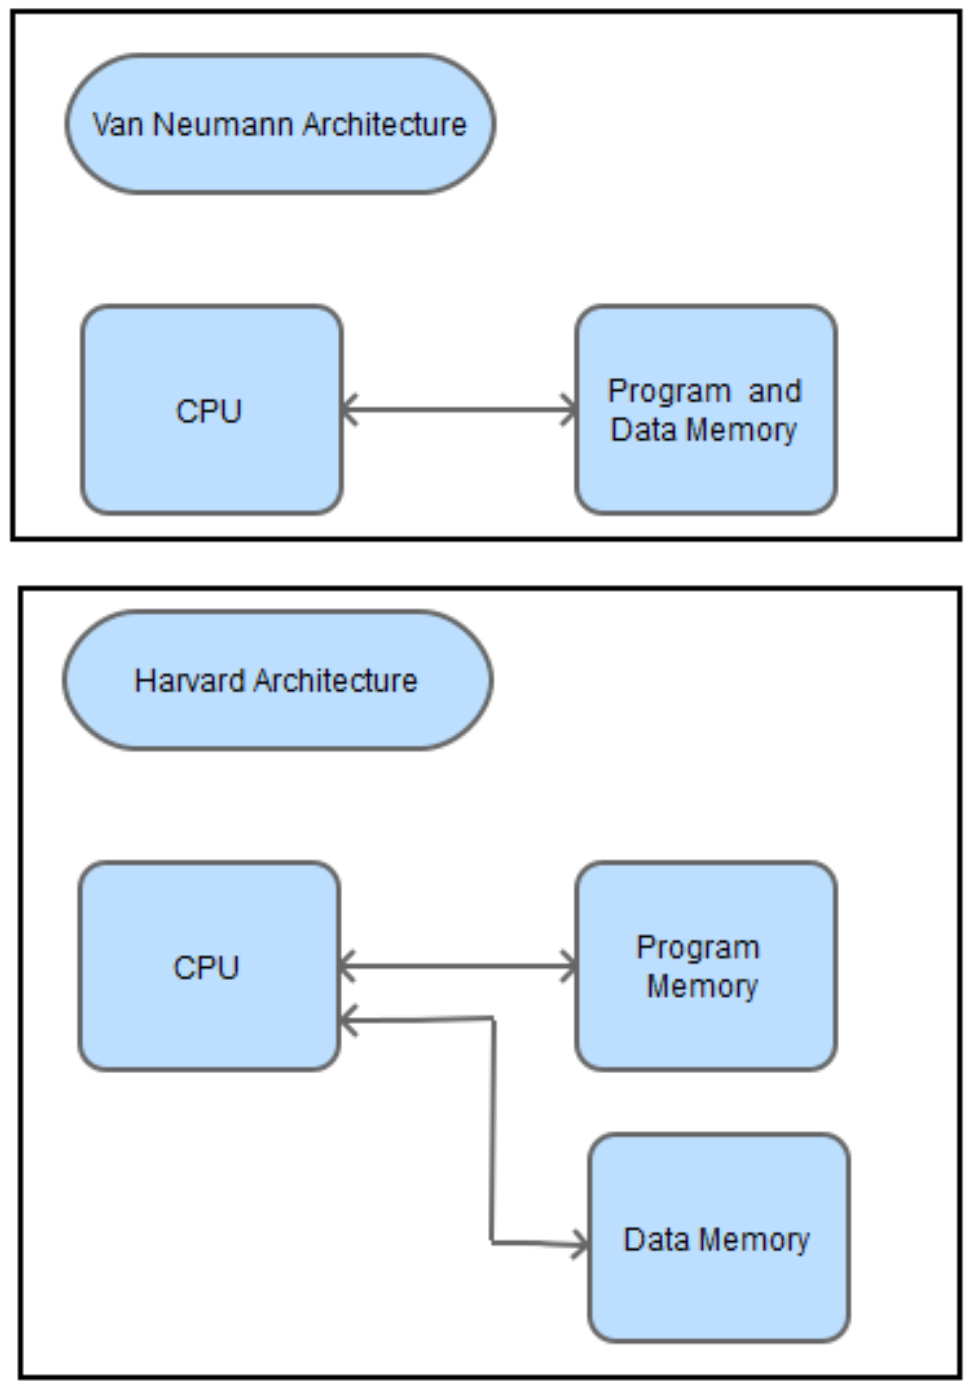
\includegraphics[width=0.4\textwidth]{neumann_vs_harvard.png}\\
\caption{Von Neumann vs Harvard Architecture}
\end{figure}

\subsection{Perbedaan CISC dan RISC}
CISC atau Complex Instruction Set Computer merupakan komputer yang mana satu instruksi dapat mengeksekusi beberapa operasi \textit{low-level} seperti load dari memori, operasi aritmatika, dan memory store atau juga melakukan addressing mode dalam satu instruksi. RISC atau Reduced Instruction Set Computer merupakan komputer yang memiliki instruksi-instruksi kecil yang teroptimasi. Ini tentu saja berbeda dari CISC yang set instruksinya lebih kompleks. 

\begin{figure}[H]
\centering
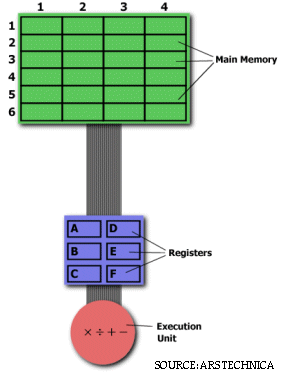
\includegraphics[width=0.5\textwidth]{memoryfig.png}\\
\caption{Diagram Memori}
\end{figure}

Gambar diatas adalah diagram dari skema penyimpanan pada komputer generik. Main memory dibagi menjadi kolom dan baris. Unit eksekusi bertugas untuk melaksanakan semua komputasi. Namun, unit eksekusi hanya dapat beroperasi pada data yang sudah ditampung pada salah satu dari 6 register. Katakanlah kita ingin mendapat hasil kali dari 2 angka. Angka pertama disimpan di lokasi 2:3, dan angka kedua di lokasi 5:2, kemudian simpan hasil kali di lokasi 2:3. Tujuan dari CISC adalah mengerjakan task dengan menggunakan baris instruksi sesedikit mungkin. Hal ini dapat dilakukan dengan prosesor yang dapat mengerti dan mengeksekusi rentetan operasi. Untuk task ini, CISC sudah dipersiapkan dengan instruksi spesifik (kita akan menyebutnya "MULT"). Ketika dieksekusi, instruksi ini akan menampung kedua nilai ke register terpisah, mengalikan operand di unit eksekusi, lalu menyimpan hasilnya di suatu register. Maka dari itu, keseluruhan task dapat diselesaikan hanya dengan 1 instruksi.

\begin{verbatim}
  MULT 2:3, 5:2
\end{verbatim}

MULT disini adalah "complex instruction". Ini adalah approach yang digunakan oleh CISC. Pada RISC, prosesor hanya melakukan instruksi sederhana yang dapat dieksekusi dalam 1 siklus clock. Maka, "MULT" command diatas dapat dibagi menjadi 3 command: "LOAD", yang memindah data dari memory ke register, "PROD", yang mengalikan operan, dan "STORE", yang memindahkan data dari register ke memory. Untuk melakukan hal yang sama dengan CISC, maka pada RISC programmer perlu menulis 4 baris assembly:

\begin{verbatim}
  LOAD A, 2:3
  LOAD B, 5:2
  PROD A, B
  STORE 2:3, A
\end{verbatim}

Dengan memisahkan instruksi "LOAD" dan "STORE" sebenarnya mengurangi beban komputasi pada komputer. Setelah instruksi "MULT" milik CISC dieksekusi, prosesor akan otomatis menghapus register. Apabila salah satu operan ingin digunakan lagi untuk komputasi lainnya, maka prosesor harus me-load lagi data dari memori ke register. Pada RISC, operan akan tetap berada di register sampai value lain diletakkan disana.

\subsection{Scheduling dari RTOS}
RTOS (Real-time operating system) adalah sebuah OS yang diperuntukkan untuk melayani real-time application yang akan memproses data saat datanya itu tiba, tanpa delay. Sistem real time ini memiliki batasan waktu untuk melakukan pemrosesan. Processing data ini harus dilakukan selama masih dalam batasan waktu yang ditentukan, jika tidak maka system akan gagal. Sebuah task memiliki 4 state, yakni Running, Ready, Blocked, dan Suspended. Ketika suatu task itu sedang berjalan, maka task itu berada dalam state Running. Artinya task tersebut sedang menggunakan prosesor. Apabila prosesor dimana RTOS berjalan hanya memiliki 1 core maka hanya 1 task saja yang dapat dieksekusi tiap waktu. Task akan berada pada state Ready jika task tersebut sudah dapat dieksekusi namun tidak dieksekusi karena task yang memiliki priority yang sama atau lebih tinggi sedang berada pada state Running. Sebuah task dikatakan dalam keadaan Blocked apabila task tersebut sedang menunggu event temporal ataupun external. Contohnya, apabila sebuah task memanggil vTaskDelay() maka akan diblok hingga delaynya selesai -sebuah event temporal. Task yang berada dalam state Blocked biasanya memiliki timeout. Task yang berada pada state blocked tidak menggunakan prosesor dan tidak dapat dipilih untuk berada dalam state Running. Seperti Blocked, task yang berada dalam state Suspended tidak dapat dipilih untuk berada dalam state Running, tetapi task yang Suspended tidak memiliki timeout. Task hanya dapat meninggalkan state Suspended dengan diperintahkan dengan API \verb|vTaskSuspend()| dan \verb|xTaskResume()|.

\begin{figure}[H]
\centering
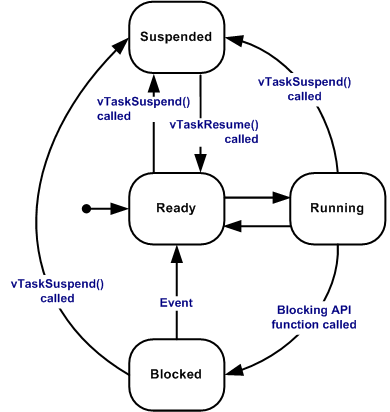
\includegraphics[width=0.5\textwidth]{taskstate.png}\\
\caption{Task State}
\end{figure}

Scheduler merupakan sebuah algoritma yang menentukan task mana yang akan dieksekusi. Pada FreeRTOS algoritma scheduling yang digunakan adalah round-robin. Round-robin ini dapat digunakan dengan scheduling preemptive atau cooperative. Pada preemptive, apabila terdapat task yang memiliki priority lebih tinggi dari task yang sedang Running, maka state dari task akan disimpan dulu di memory, kemudian prosesor akan menjalankan task dengan priority yang lebih tinggi dahulu. Setelah itu, maka task sebelumnya akan dijalankan kembali. Hal ini dinamakan sebagai context switching. Pada cooperative scheduling, task yang sedang berjalan tidak dapat dihentikan sebelum tasknya selesai dieksekusi. Ketika terdapat task dengan priority lebih tinggi, maka scheduler akan mengeksekusinya setelah task yang sedang berjalan selesai.

\end{document}
